During this assignment, the setup in Figure \ref{fig:Ass1_setup} is used. It consists of a klystron-based generator (control block) which provides the necessary voltages and modulations for a microwave with a frequency of around 9.1 GHz. The generator is connected to a horn antenna, which can rotate along the direction of transmission, transmitting a linearly polarised wave. Rotating the antenna means the direction of polarisation will also be rotated.\\
This antenna is also present on the receiving end of the experimental setup. The signal received by this antenna is picked up by a detector, which converts the amplitude of the received signal into a low-frequency signal for further amplification and measurement, which is done with a voltmeter. Because the detector is a quadratic detector, the measured voltage of the voltmeter is proportional to the amplitude of the received signal.\\

\begin{figure}[h]
    \centering
    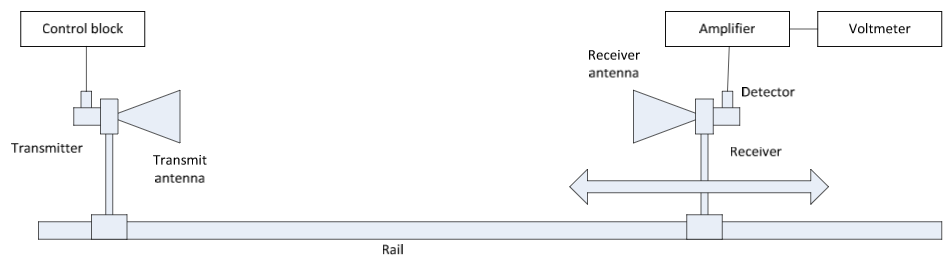
\includegraphics[width=1\textwidth]{Session2_files/Assignment1_setup.PNG}
    \caption{Experimental setup of Assignment 1, taken from [1].}
    \label{fig:Ass1_setup}
\end{figure}

\subsection*{Propagation Velocity in Free Space}

For this experiment, an array of parallel conducting rods is inserted in between the transmitting and receiving antenna, creating a standing wave. Moving the location of the array, the signal will be amplified or attenuated according to antinodes and nodes of the wave, respectively.\\
By measuring the distance between two nodes or two antinodes, the wavelength can be calculated, which, combined with the given frequency results in the propagation velocity of the wave.\\

The distances between five successive nodes were measured, after which an average of these values was taken as the half wavelength of the wave. The measured distances can be seen in Table \ref{tab:Ass1}. From these values, a wavelength of about $32.5$ mm was found, which results in a propagation velocity of $u_p = \lambda f = 32.5\cdot10^{-3} \cdot 9.1\cdot 10^9 = 295.75\cdot10^6 \frac{m}{s}$. This is $1.3\%$ lower than the speed of light c, which can be due to measurement errors, or the frequency of the generator not being precise.

\begin{table}[h]
\centering
\caption{Distances between successive nodes.}
\label{tab:Ass1}
\begin{tabular}{|l|c|c|}
\hline
      & \multicolumn{1}{l|}{d {[}mm{]}} & \multicolumn{1}{l|}{$\Delta d$ {[}mm{]}} \\ \hline
$n_1$ & 1075                            &                                          \\ \hline
$n_2$ & 1091                            & 16                                       \\ \hline
$n_3$ & 1108                            & 17                                       \\ \hline
$n_4$ & 1123                            & 15                                       \\ \hline
$n_5$ & 1140                            & 17                                       \\ \hline
\end{tabular}
\end{table}

\subsection*{Free Space Attenuation}

In an perfect vacuum, an EM wave would not be attenuated, but since the experiment is not conducted in a perfect vacuum, there will be some attenuation. The attenuation is assumed to be according to following equation:

\begin{equation*}
    A_w = \frac{C}{R^x}
\end{equation*}

where $A_w$ is the amplitude of the measured signal, $C$ a constant and $R$ the distance between the transmitter and receiver. The amplitude of the signal was measured at 9 different distances from the transmitter, as seen in Table \ref{tab:Ass1_2}. Filling in these values in the assumed equation results in values of $C \approx 0.55 V^{-1}m^{-2}$ and $x \approx 2.7245$.

\begin{table}[h]
\centering
\caption{Amplitudes of the wave for different distances.}
\label{tab:Ass1_2}
\begin{tabular}{l|lllllllll}
d {[}m{]} & 0.80 & 0.85  & 0.90  & 0.95  & 1.00  & 1.05  & 1.10  & 1.15  & 1.20  \\ \hline
A {[}V{]} & 0.94 & 0.835 & 0.700 & 0.608 & 0.536 & 0.460 & 0.407 & 0.359 & 0.317
\end{tabular}
\end{table}

As EM waves attenuate according to the inverse square law, $x=2$ should result from this experiment. However, the calculated value is far from this value. In Figure \ref{fig:Ass1_AvsD}, the measured values and the predicted values are plotted. This difference might be explained by measurement errors, and by the small distance along which the amplitudes were measured. A better estimation of $x$ would result if the distance over which measurements are performed was larger.

\begin{figure}[h]
    \centering
    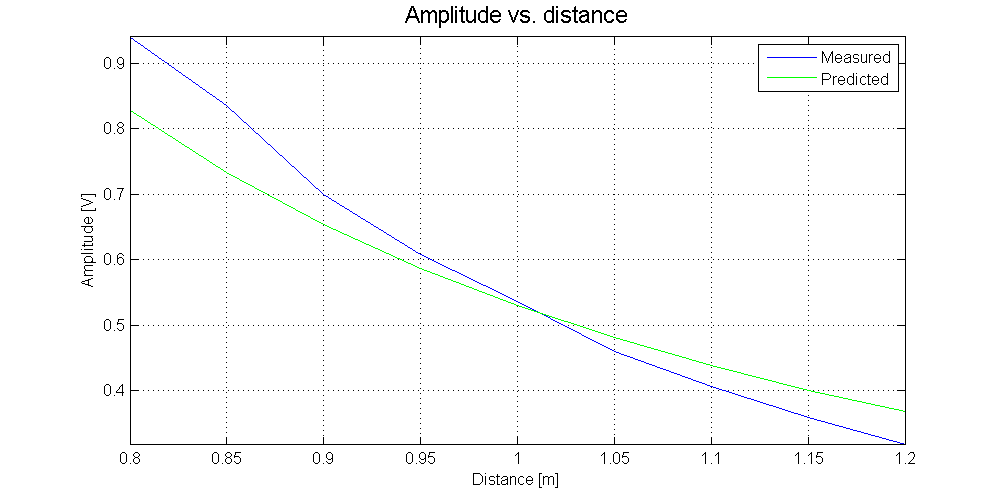
\includegraphics[width=1\textwidth]{Session2_files/AvsD.png}
    \caption{Wave amplitude versus distance.}
    \label{fig:Ass1_AvsD}
\end{figure}

\subsection*{Transmission and Absorption of EM waves}

In this experiment, the propagation of a vertically polarised wave when a medium is present in between the transmitter and receiver, is investigated. In order to conduct this experiment, the antennas were oriented so that the polarisation would be vertical. The distance between the transmitter and receiver was fixed to a certain distance of about $1.5m$ throughout the experiment, while the media were placed at about $30cm$ of the transmitting antenna. The amplitudes measured at the receiver can be seen in Table \ref{tab:Ass1_3}.

\begin{table}[h]
\centering
\caption{Wave amplitudes for different media.}
\label{tab:Ass1_3}
\begin{tabular}{|l|c|c|}
\hline
Medium             & \multicolumn{1}{l|}{Amplitude {[}V{]}} & \multicolumn{1}{l|}{Amplitude {[}dB{]}} \\ \hline
Air                & 0.143                                  & 0                                       \\ \hline
Metal sheet        & 0.019                                  & -17.5                                   \\ \hline
Dielectric plate   & 0.122                                  & -1.38                                   \\ \hline
Absorbing material & 0.018                                  & -18.0                                   \\ \hline
Array (horizontal) & 0.155                                  & 0.700                                   \\ \hline
Array (vertical)   & 0.016                                  & -19.0                                   \\ \hline
\end{tabular}
\end{table}

By comparing the measured voltage, which is proportional to the power of the received wave, with the voltage measured when no medium is present, the absorbing or insulating properties of the media can be discussed.

\begin{itemize}
    \item It can be seen that the metal sheet absorbs most of the transmitted power. This is due to the fact that no electric field can be present in a good conductor (the metal plate short circuits the field), so there will be no electric field present to be measured behind the plate.
    
    \item In contrast to the metal sheet, the dielectric plate does not short the electric field, which means there will be an electric field in the dielectric plate. This field is again transmitted from the back side of the plate, which can be verified by the amplitude only slightly being attenuated.
    
    \item The absorbing material basically absorbs the electric field, reducing the electric field in the medium to almost zero, which can be seen by an attenuation of about $-18 dB$.
    
    \item While the amplitude of the wave seems to be amplified due to the array of parallel conducting rods in a horizontal orientation, this cannot be the case in reality. The amplification of $0.7dB$ is most likely due to measurement error. It is expected however, that the attenuation will be very low.
\end{itemize}